\documentclass[12pt]{report}
\usepackage[utf8]{inputenc}
\usepackage[T1]{fontenc}
\usepackage[french]{babel}
\usepackage{graphicx} 
\usepackage{amsmath}
\usepackage{hyperref}
\usepackage{float}
\usepackage{geometry}
\geometry{
 a4paper,
 left=15mm,
 top=20mm,
 right=15mm
 }

% Configuration de hyperref pour que les liens ne soient pas entourés de cadres rouges
\hypersetup{
    colorlinks=true,
    linkcolor=black,
    urlcolor=blue
}

% Définition de la ligne horizontale
\newcommand{\HRule}{\rule{\linewidth}{0.5mm}}
\renewcommand{\thesection}{\arabic{section}}
\renewcommand{\thesubsection}{\thesection.\arabic{subsection}}

\begin{document}

\begin{titlepage}
    \centering
    
    \vspace*{2cm}
    
    \textsc{\Large Rapport de Projet}\\[0.5cm]
    \textsc{\large UE : Graph Theory IMT ATLANTIQUE}\\[2cm]
    
    \HRule \\[0.4cm]
    {\huge \bfseries  Challenge 2 }\\[0.2cm]
    {\large \textit{Reddit moderation - DSA Compliance Analysis}}\\[0.4cm]
    \HRule \\[2cm] % Espace réduit ici pour équilibrer

    % Lien GitHub cliquable placé au-dessus des auteurs
    {\large \textbf{Dépôt GitHub :}} \\[0.2cm]
    {\small \url{https://github.com/LucRobey/Graph_Theory_Challenge_2.git}} \\[1.5cm]
    
    {\large \emph{Auteurs :}}\\[0.5cm]
    {\Large Camille \textsc{Azéma}}\\[0.2cm]
    {\Large Luc \textsc{Robey}}
    
    \vfill  
    {\large Mars 2026}
    
\end{titlepage}

\renewcommand{\contentsname}{Sommaire}
\tableofcontents
\newpage

\section{Introduction}
L'objectif de ce projet est d'explorer les dynamiques d'interaction au sein de communautés Reddit afin d'identifier des comportements malveillants, des tentatives de manipulation ou des acteurs d'influence disproportionnée. 

\section{Compréhension du problème métier}
\subsection{Contexte et enjeux}
L'entrée en vigueur du \textit{Digital Services Act} (DSA) impose à Reddit de passer d'une modération réactive à une posture proactive. L'enjeu pour la direction de la modération est triple :
\begin{itemize}
    \item \textbf{Légal :} Éviter des sanctions financières pouvant atteindre 6 \% du chiffre d'affaires mondial.
    \item \textbf{Éthique :} Protéger la communauté en réduisant le temps d'exposition aux contenus toxiques.
    \item \textbf{Opérationnel :} Optimiser l'efficacité des Community Managers en automatisant la détection des cas triviaux pour réduire leur charge mentale.
\end{itemize}

\subsection{Modélisation du problème}
La détection de la malveillance est traduite en une tâche de caractérisation de structures relationnelles via la théorie des graphes. Nous modélisons les interactions comme un graphe orienté $\mathcal{G} = (V, E)$ où :
\begin{itemize}
    \item $V$ (Nœuds) représente l'ensemble des utilisateurs.
    \item $E$ (Arêtes) représente les interactions (réponses aux posts/commentaires).
\end{itemize}
\textbf{Hypothèse :} La propagation de contenus nocifs se manifeste par des propriétés topologiques spécifiques, telles que des densités locales anormales ou l'émergence de "hubs" d'influence polarisés.

\subsection{Objectifs Data Science et plan d'action}
La stratégie de réponse repose sur trois axes techniques :
\begin{itemize}
    \item \textbf{Détection de communautés :} Algorithme de clustering (Louvain) pour isoler des sous-groupes suspects.
    \item \textbf{Identification des acteurs pivots :} Utilisation des mesures de centralité (\textit{Betweenness} et \textit{PageRank}) pour repérer les vecteurs de diffusion.    
    \item \textbf{Analyse temporelle :} Repérage des pics de densité signalant des campagnes de manipulation coordonnées.
\end{itemize}

\subsection{Critères de réussite et risques}
La performance de la solution est évaluée sur sa capacité à identifier des phénomènes de propagation anormaux via :
\begin{itemize}
    \item \textbf{La robustesse :} Isolation de sous-graphes dont la densité est significativement supérieure à la moyenne du réseau.
    \item \textbf{La centralité d'alerte :} Identification des nœuds $v \in V$ possédant une forte intermédiarité, agissant comme ponts de désinformation.
\end{itemize}
\textbf{Risques :} Le projet doit arbitrer entre les \textbf{Faux Positifs} (risque de censure/frein à l'engagement) et les \textbf{Faux Négatifs} (non-respect de la loi par défaut de détection).

\section{Collecte et nettoyage des données}
\subsection{Sources de données}
Nous avons utilisé deux fichiers principaux : \texttt{all\_posts\_active\_subreddit.csv} et \texttt{all\_comments.csv}. Ces fichiers contiennent l'historique des publications et des commentaires, capturant la richesse des échanges entre utilisateurs.

\subsection{Prétraitement temporel}
Pour l'analyse dynamique, nous avons converti les horodatages au format \texttt{ISOYearWeek} (ex: 2024-W12), permettant de discrétiser le graphe en fenêtres hebdomadaires. Cette approche est cruciale pour observer l'évolution de la topologie du réseau et détecter des pics d'activité suspects.

\subsection{Suppression des comptes inactifs et bots}
Un nettoyage a été effectué sur ces deux points :
\begin{itemize}
    \item \textbf{Comptes supprimés} : Plus de 17 000 comptes marqués comme \texttt{[deleted]} ont été retirés. Ces comptes, bien qu'ayant contribué par le passé, ne font plus partie du réseau social actif.
    \item \textbf{Bots et automoderator} : Environ 2 500 interactions provenant de bots automatisés ont été filtrées via une liste noire.
\end{itemize}

\begin{figure}[H]
    \centering
    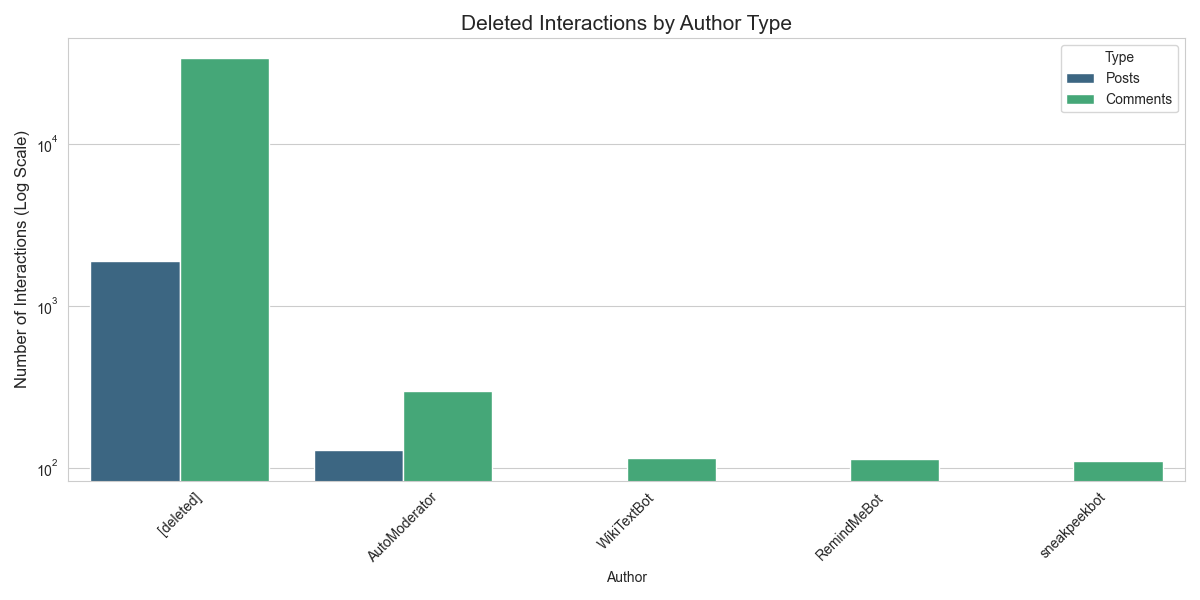
\includegraphics[width=0.7\textwidth]{images/deleted_authors_bar.png}
    \caption{Volumes d'auteurs supprimés par subreddit, mettant en évidence les zones de forte instabilité.}
    \label{fig:deleted_authors}
\end{figure}

\section{Préparation des données}
\subsection{Construction du graphe d'interaction}
Le graphe est construit de manière à ce que chaque arête représente une interaction directe (réponse). Si l'utilisateur A commente une publication de B, ou répond à un commentaire de B, une arête dirigée est créée de A vers B. 

\subsection{Calcul des poids}
Afin de ne pas traiter toutes les interactions de manière identique, nous avons introduit une pondération basée sur la richesse du contenu échangé. 
Le poids $w_{i,j}$ d'une arête est calculé selon la formule suivante : 
\begin{equation}
    w = \text{base} + \frac{\text{longueur du contenu}}{1000}
\end{equation}
La valeur de base est fixée à $2,0$ pour une réponse à une publication et à $1,0$ pour une réponse à un commentaire. Cette pondération permet de valoriser les interactions riches en information tout en distinguant l'importance hiérarchique des réponses.

\section{Modélisation de la solution}
\subsection{Analyse de centralité}
Nous utilisons d'abord l'algorithme de Louvain dans l'objectif de réaliser un clustering afin de détecter les différentes communautés présentes dans le réseau social. Ensuite, afin d'identifier les piliers de la communauté ainsi que les intermédiaires stratégiques, nous calculons deux métriques :
\begin{itemize}
    \item \textbf{PageRank (Centralité d'autorité)} : Mesure l'influence organique. Un score PageRank élevé indique un utilisateur dont les contributions sont validées par d'autres acteurs influents.
    \item \textbf{Betweenness (Centralité d'intermédiarité)} : Identifie les "ponts" entre sous-groupes. Ces nœuds sont critiques pour la propagation de l'information et peuvent représenter des modérateurs ou des profils cherchant à infiltrer plusieurs communautés.
\end{itemize}

\subsection{Décomposition $k$-core (Structure Core-Periphery)}
Cette technique permet de séparer le "backbone" (noyau dur) des utilisateurs périphériques. Un utilisateur appartient au $k$-core s'il est connecté à au moins $k$ autres utilisateurs du même niveau. Le cœur du réseau représente les interactions les plus stables et les plus denses.

\subsubsection{Modélisation Core-Periphery}
Afin de distinguer les utilisateurs plus fréquents du réseau des participants occasionnels, nous appliquons une décomposition par $k$-core. C'est un algorithme qui identifie les sous-graphes cohésifs en retirant itérativement les nœuds de plus faible degré jusqu'à ce que le graphe soit vide.

\begin{itemize}
    \item \textbf{Le core (noyau)} : Défini par les nœuds situés au-delà du 90ème percentile du niveau de coreness ($x \geq \text{quantile}(0.9)$).
    \item \textbf{La périphérie} : Utilisateurs ayant un faible degré d'engagement ou des liens très dispersés.
\end{itemize}

\subsection{Analyse temporelle pour chaque subreddit}
Nous avons calculé, pour chaque subreddit et chaque semaine certaines métriques qui nous aident dans la partie suivante à définir des "grades".
\begin{figure}[H]
    \centering
    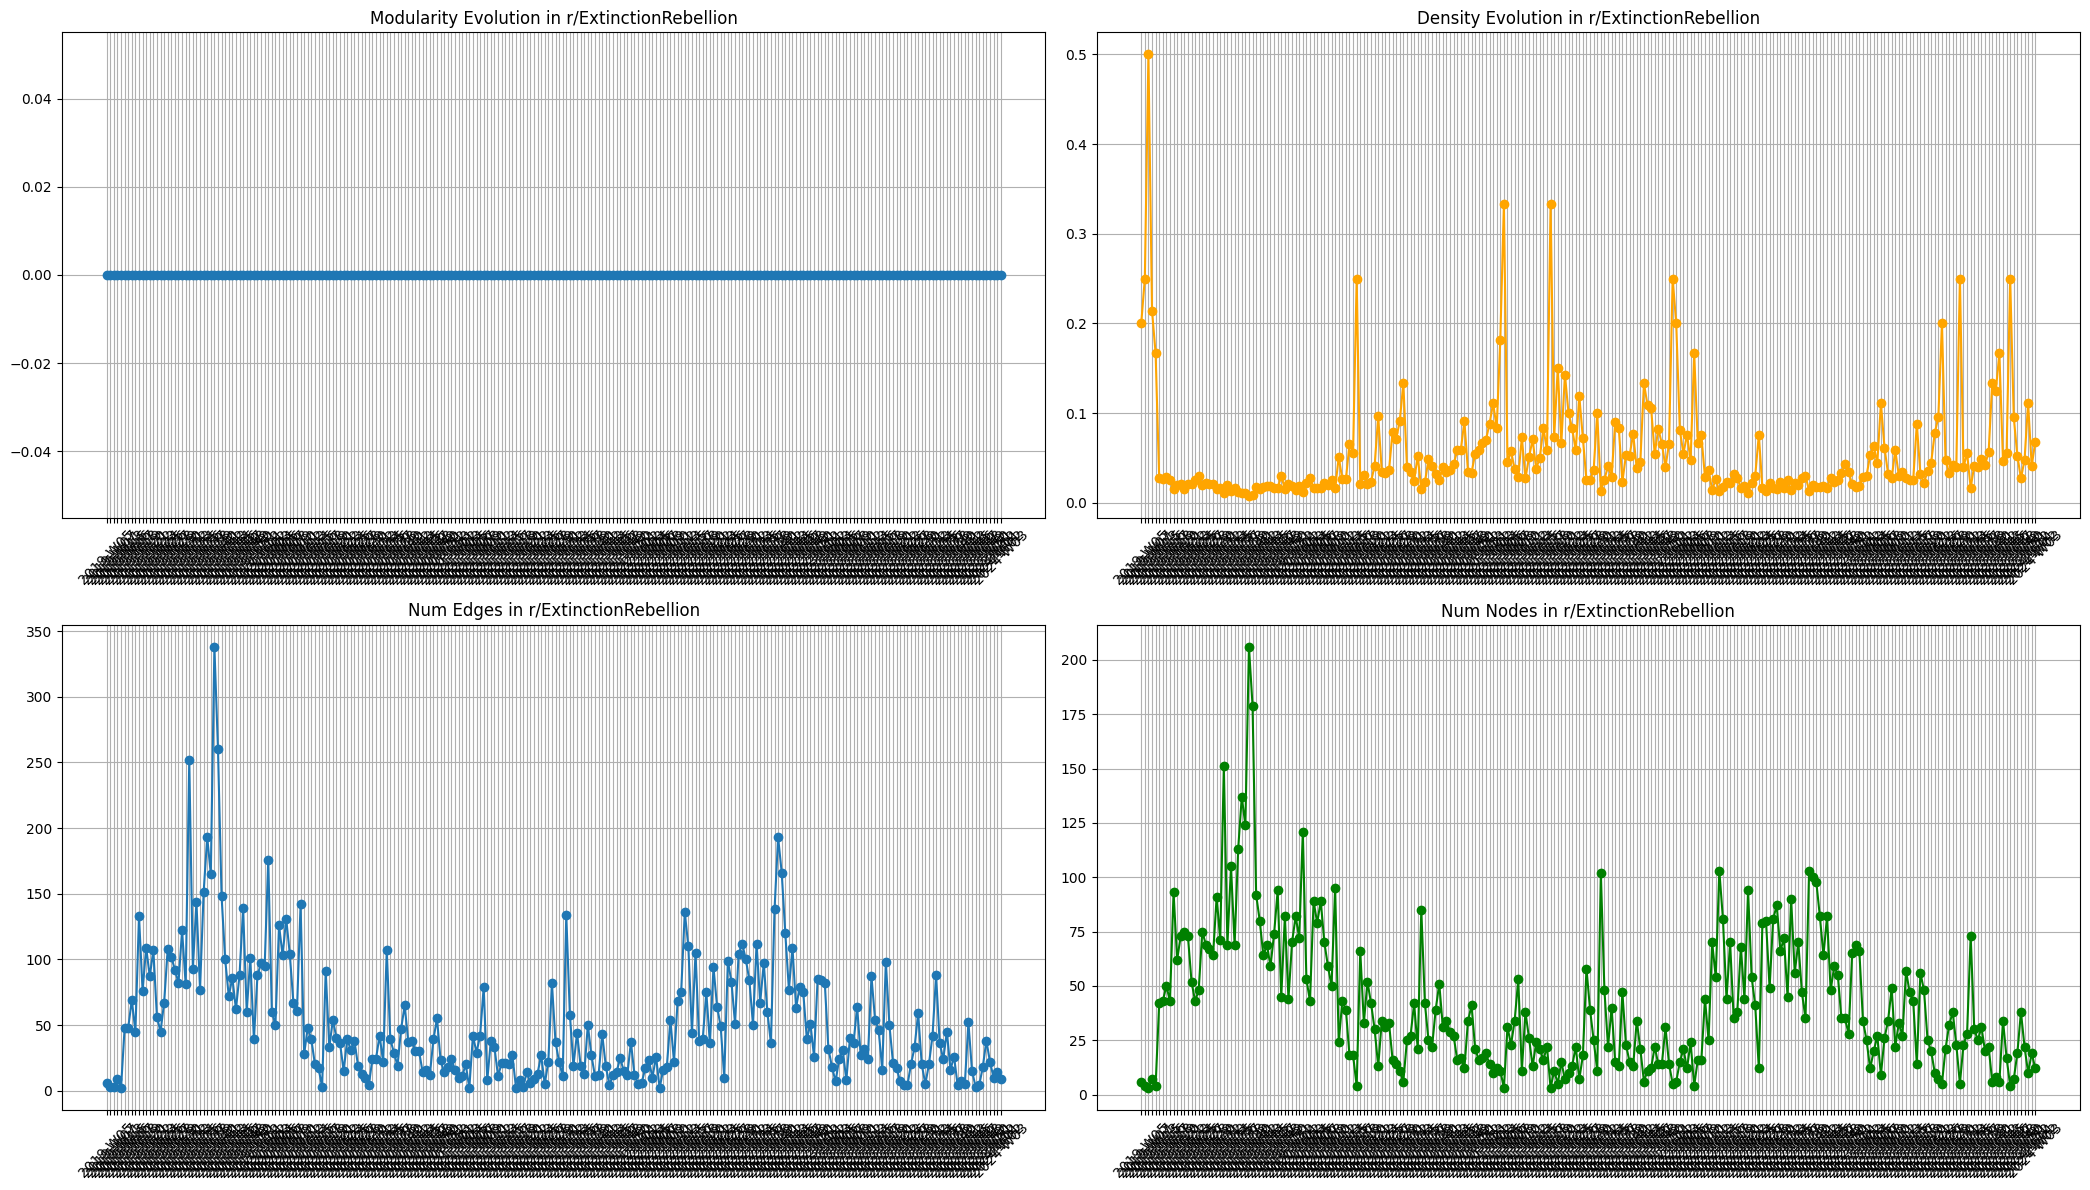
\includegraphics[width=0.65\textwidth]{images/dynamic_subreddits.png}
    \caption{Exemple d'analyse dynamique d'un subreddit.}
    \label{fig:grades}
\end{figure}

\subsection{Analyse comportementale dynamique}
Nous avons implémenté un système de notation à sept dimensions pour grader le comportement des utilisateurs :
\begin{enumerate}
    \item \textbf{Spammer ratio} (Sortant/Entrant).
    \item \textbf{Artificial bridger} (Betweenness vs PageRank).
    \item \textbf{Peripheral yeller} (Degré élevé mais Coreness faible).
    \item \textbf{Sudden leader} (Changement brusque de PageRank).
    \item \textbf{Burstiness} (Volatilité hebdomadaire de l'activité).
    \item \textbf{Instability} (Leaders émergeant lors de crises structurelles).
    \item \textbf{Coordinated Bot Ring} (Combinaison de transitivité et coreness).
\end{enumerate}

\begin{figure}[H]
    \centering
    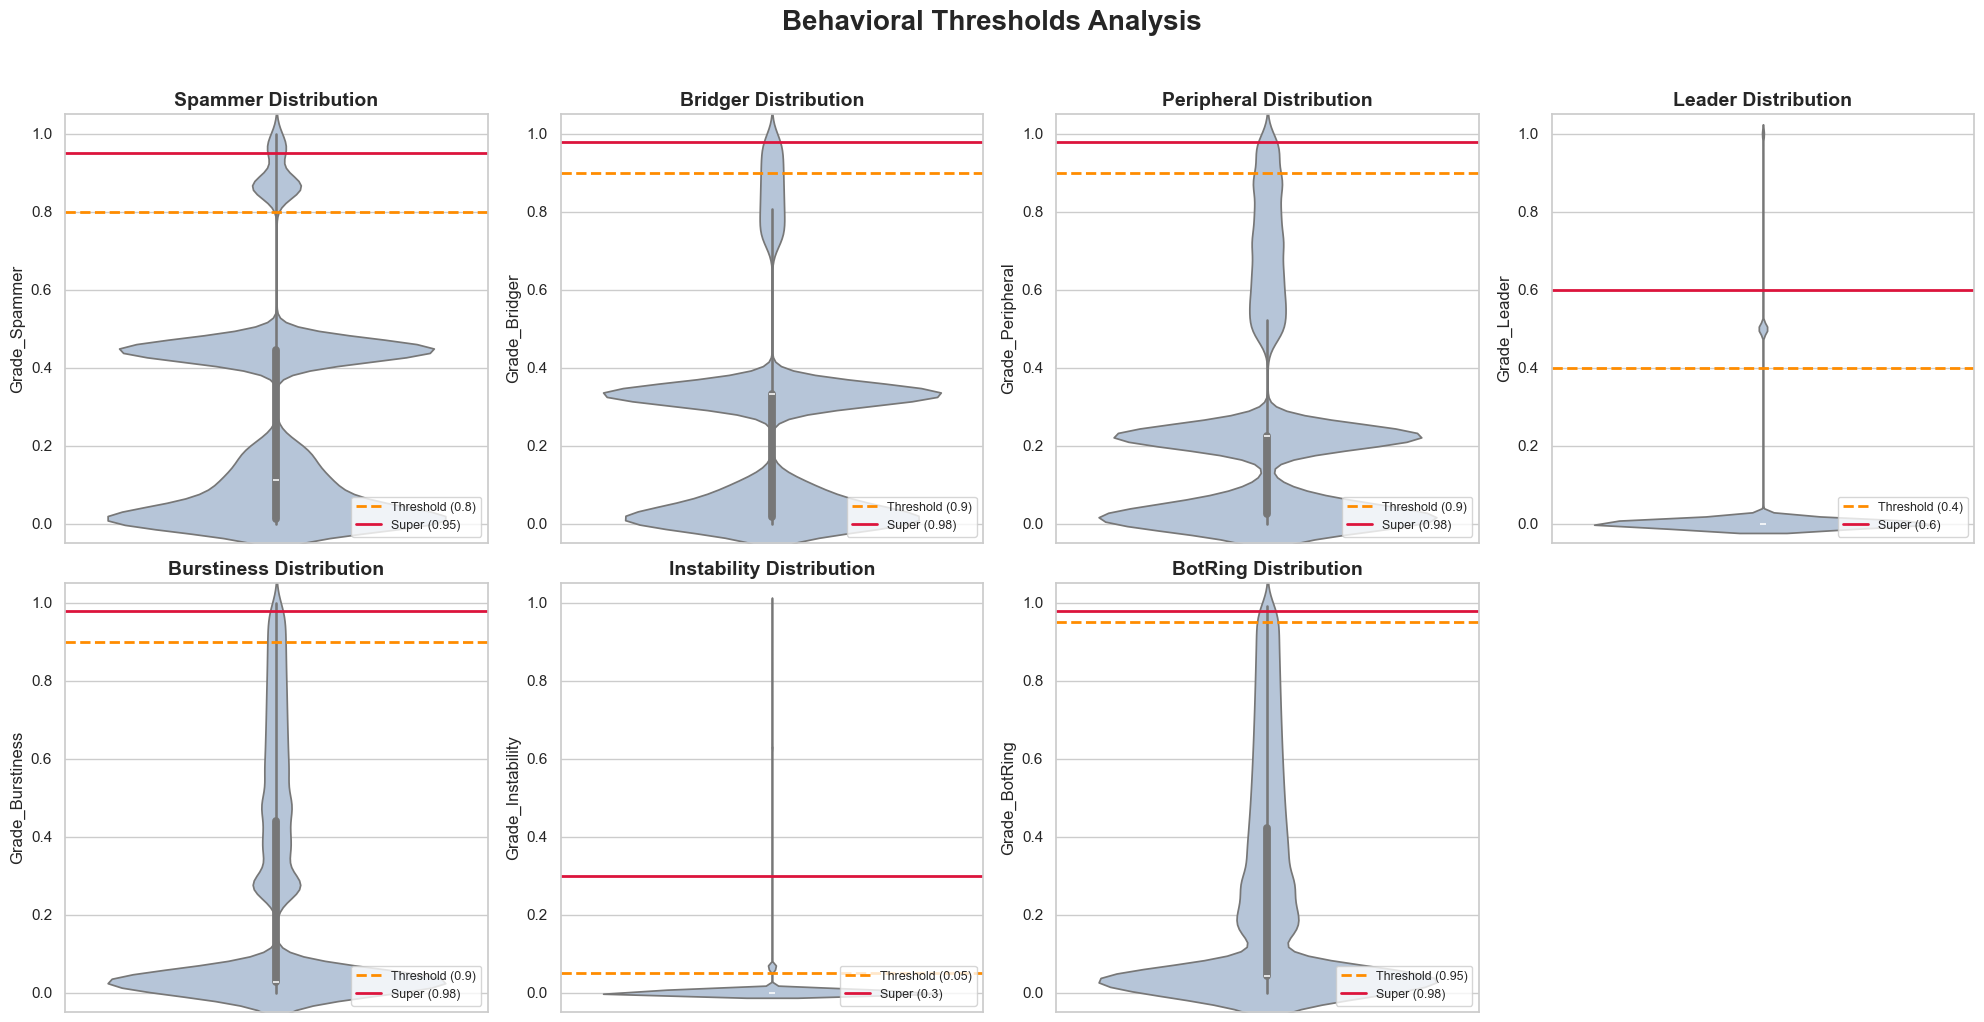
\includegraphics[width=0.8\textwidth]{images/grades_violin.png}
    \caption{Distribution des grades comportementaux, montrant les queues de distribution correspondant aux anomalies.}
    \label{fig:grades}
\end{figure}
\newpage
\section{Détection d'anomalies : comparaison des approches}
Nous avons utilisé deux méthodes de détection.

\subsection{Heuristiques topologiques (Alert Users)}
\begin{enumerate}
    \item \textbf{Le "Bridge Troll"} :
    \begin{itemize}
        \item \textbf{Critères fixés} : $Betweenness > P_{80}$ ET $PageRank < P_{20}$.
        \item \textbf{Interprétation} : C'est un utilisateur qui contrôle le flux d'information entre deux mondes, mais que personne "d'important" ne suit ou ne valide. C'est le profil typique d'un compte qui relie des chambres d'écho pour propager une fake news ou coordonner un raid.
    \end{itemize}
    
    \item \textbf{Le "Suspicious Core Member"} :
    \begin{itemize}
        \item \textbf{Critères fixés} : $Coreness\_Level = 1.0$ (Normalisé) ET $PageRank < 0.05$.
        \item \textbf{Interprétation} : C'est un compte qui est niché au cœur du réseau le plus dense, mais qui n'a aucune autorité propre. C'est souvent le signe d'une "ferme de bots" : ils sont tous très connectés entre eux (comme l'indique de Coreness élevé), mais personne à l'extérieur du groupe de bots ne les suit (ils ont une PageRank faible).
    \end{itemize}
\end{enumerate}

\subsection{Scoring multi-dimensionnel (Anomalous Users)}
Cette approche dynamique agrège les sept grades mentionnés précédemment dans un score d'anomalie total. Un système de "Red Flags" (votes) est utilisé : un utilisateur est flaggé s'il cumule plusieurs comportements suspects simultanément. Cette méthode est plus robuste car elle capte des signaux faibles (ex: burstiness) invisibles pour les heuristiques statiques.
\newline
\begin{figure}[H]
    \centering
    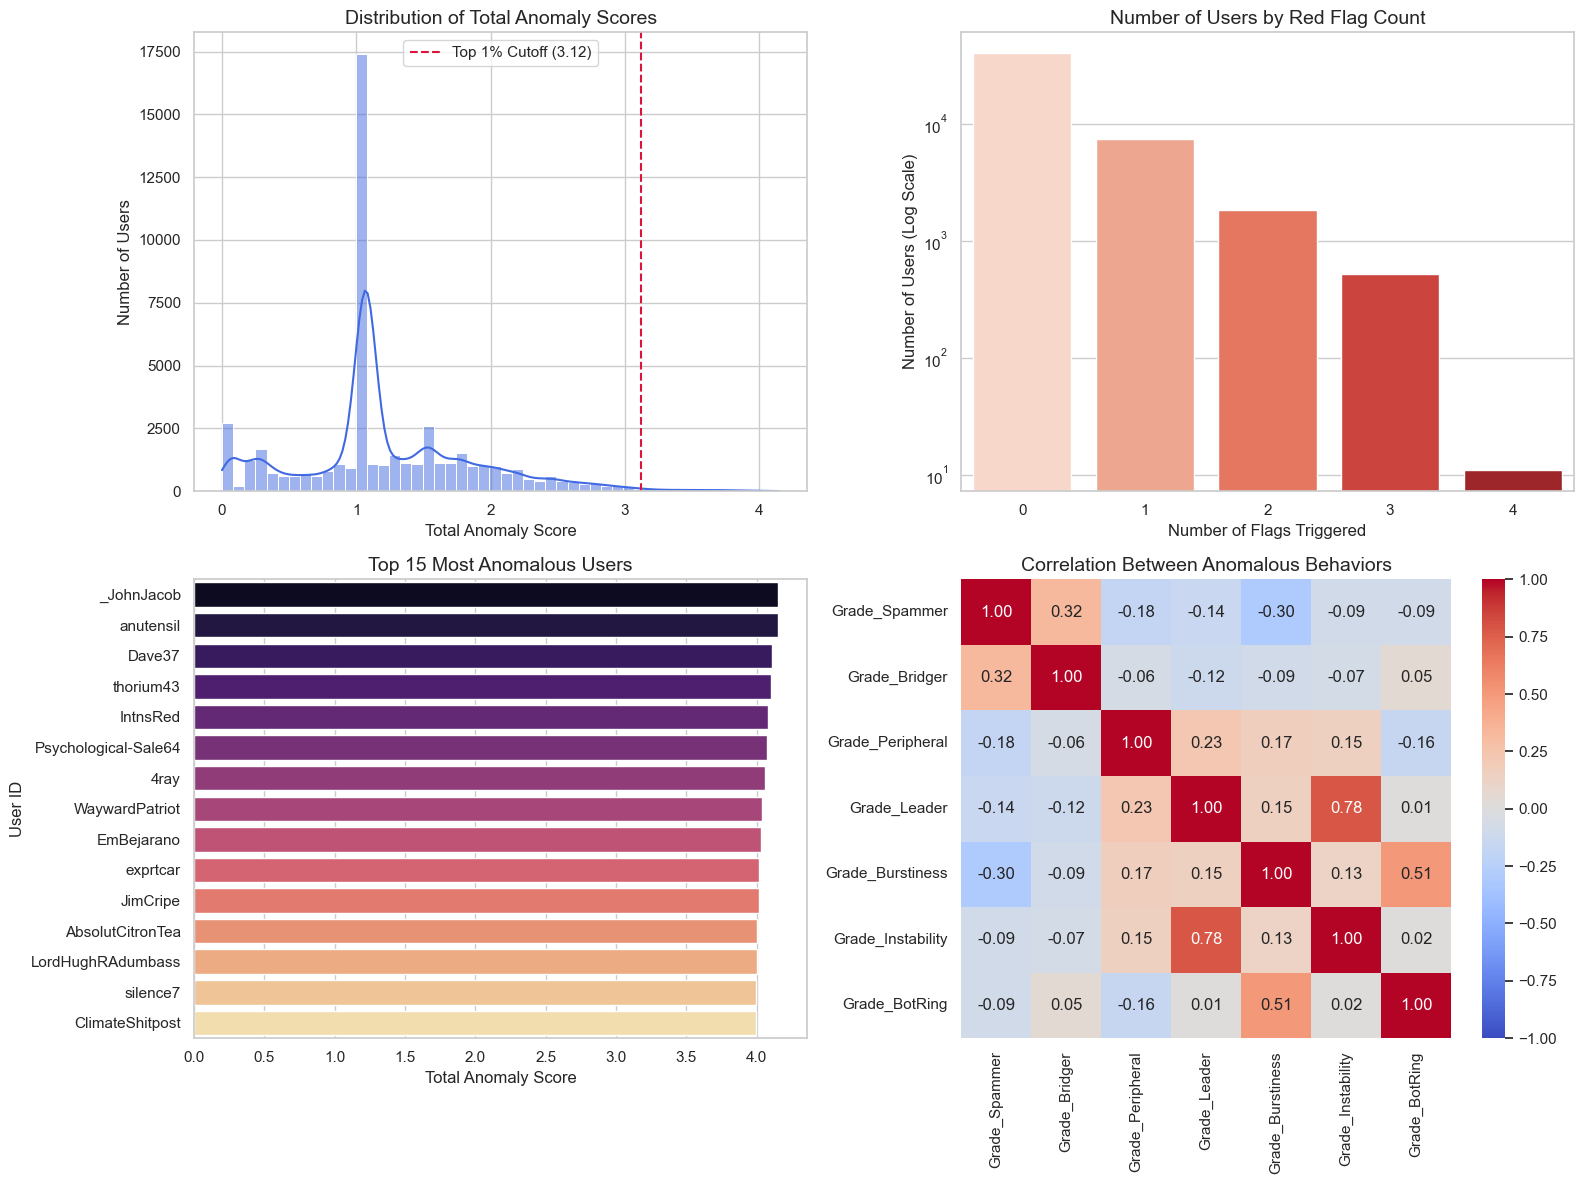
\includegraphics[width=0.9\textwidth]{images/anomaly_panel.png}
    \caption{Comparaison des différentes grades.}
    \label{fig:sentiment}
\end{figure}

Nous pouvons ainsi détecter selon une logique assez simple, basée sur la note globale ou si certaines notes sont anormalement trop élevées.
\begin{figure}[H]
    \centering
    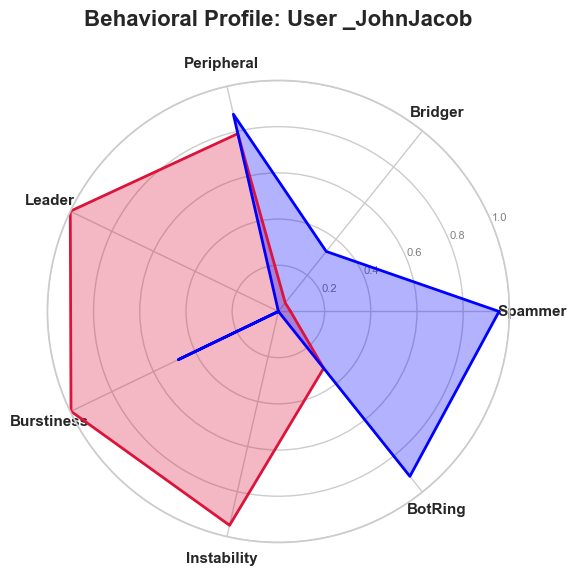
\includegraphics[width=0.45\textwidth]{images/anomalous_behavior.png}
    \caption{Exemples de profils suspects.}
    \label{fig:sentiment}
\end{figure}
\section{Évaluation de la solution}
\subsection{Test de robustesse par fragmentation}
En simulant la suppression des acteurs identifiés comme critiques (Core), le réseau subit une fragmentation majeure avec une chute de \textbf{69,53\%} de la taille de sa composante géante. Cela valide notre identification des piliers structurels.

\subsection{Amélioration de la modularité}
Le retrait des utilisateurs identifiés comme anomalies (Scoring Multi-dimensionnel) améliore la modularité du graphe de \textbf{0,25\%}. Bien que faible, cette hausse indique que les anomalies agissent comme un "bruit" structurel floutant les frontières entre communautés organiques.

\subsection{Validation par sentiment analysis}
L'analyse VADER révèle que les \textit{Anomalous Users} possèdent un sentiment moyen nettement plus négatif que le reste de la population, confirmant la corrélation entre structure de graphe suspecte et contenu toxique.

\begin{figure}[H]
    \centering
    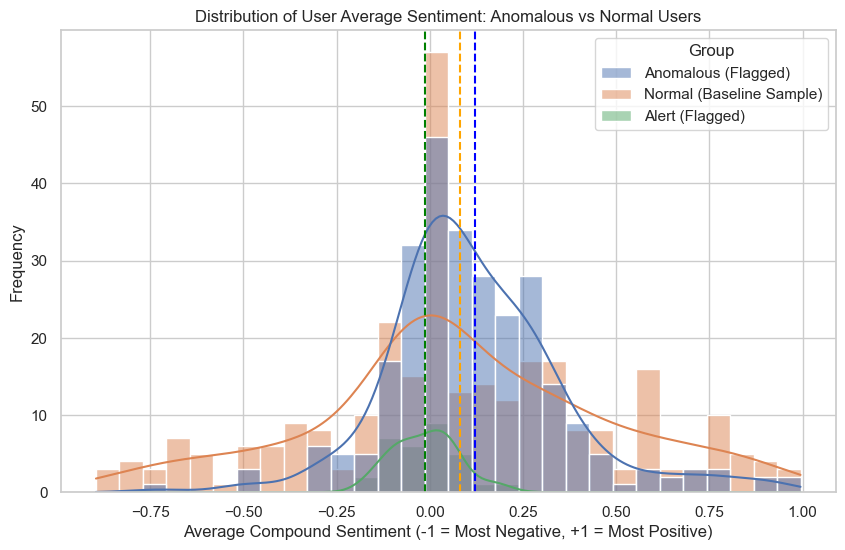
\includegraphics[width=0.7\textwidth]{images/sentiment.png}
    \caption{Corrélation entre profil d'anomalie graphique et toxicité sémantique.}
    \label{fig:sentiment}
\end{figure}

\section{Conclusion}
L'alliance des métriques topologiques classiques et d'un scoring comportemental dynamique permet une surveillance fine du réseau Reddit. Les "Alert Users" identifient les menaces structurelles immédiates, tandis que les "Anomalous Users" révèlent des stratégies de manipulation plus subtiles. Ces résultats offrent une feuille de route pour une modération ciblée et proportionnée, en adéquation avec les principes du DSA.
\begin{figure}[H]
    \centering
    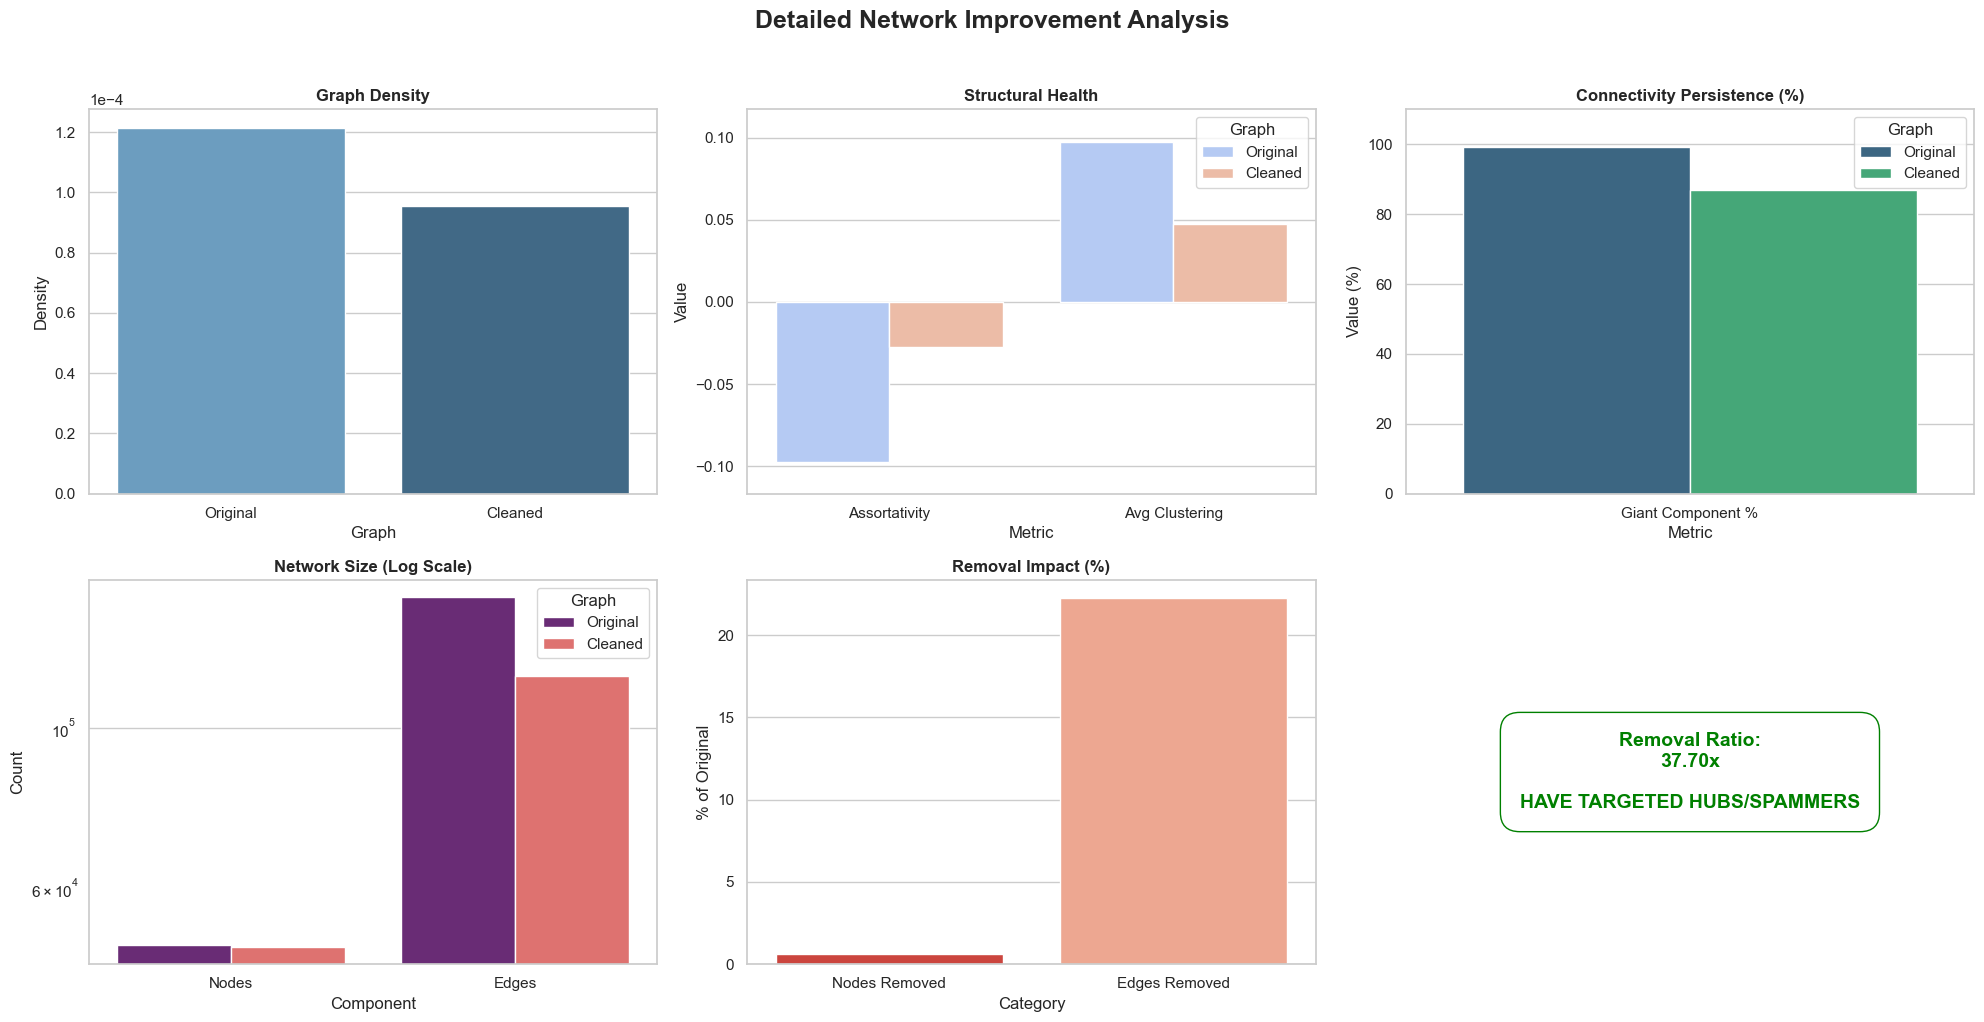
\includegraphics[width=1.0\textwidth]{images/anomalous_results.png}
    \caption{Résultats pour suppression des anomalous users.}
    \label{fig:sentiment}
\end{figure}
\begin{figure}[H]
    \centering
    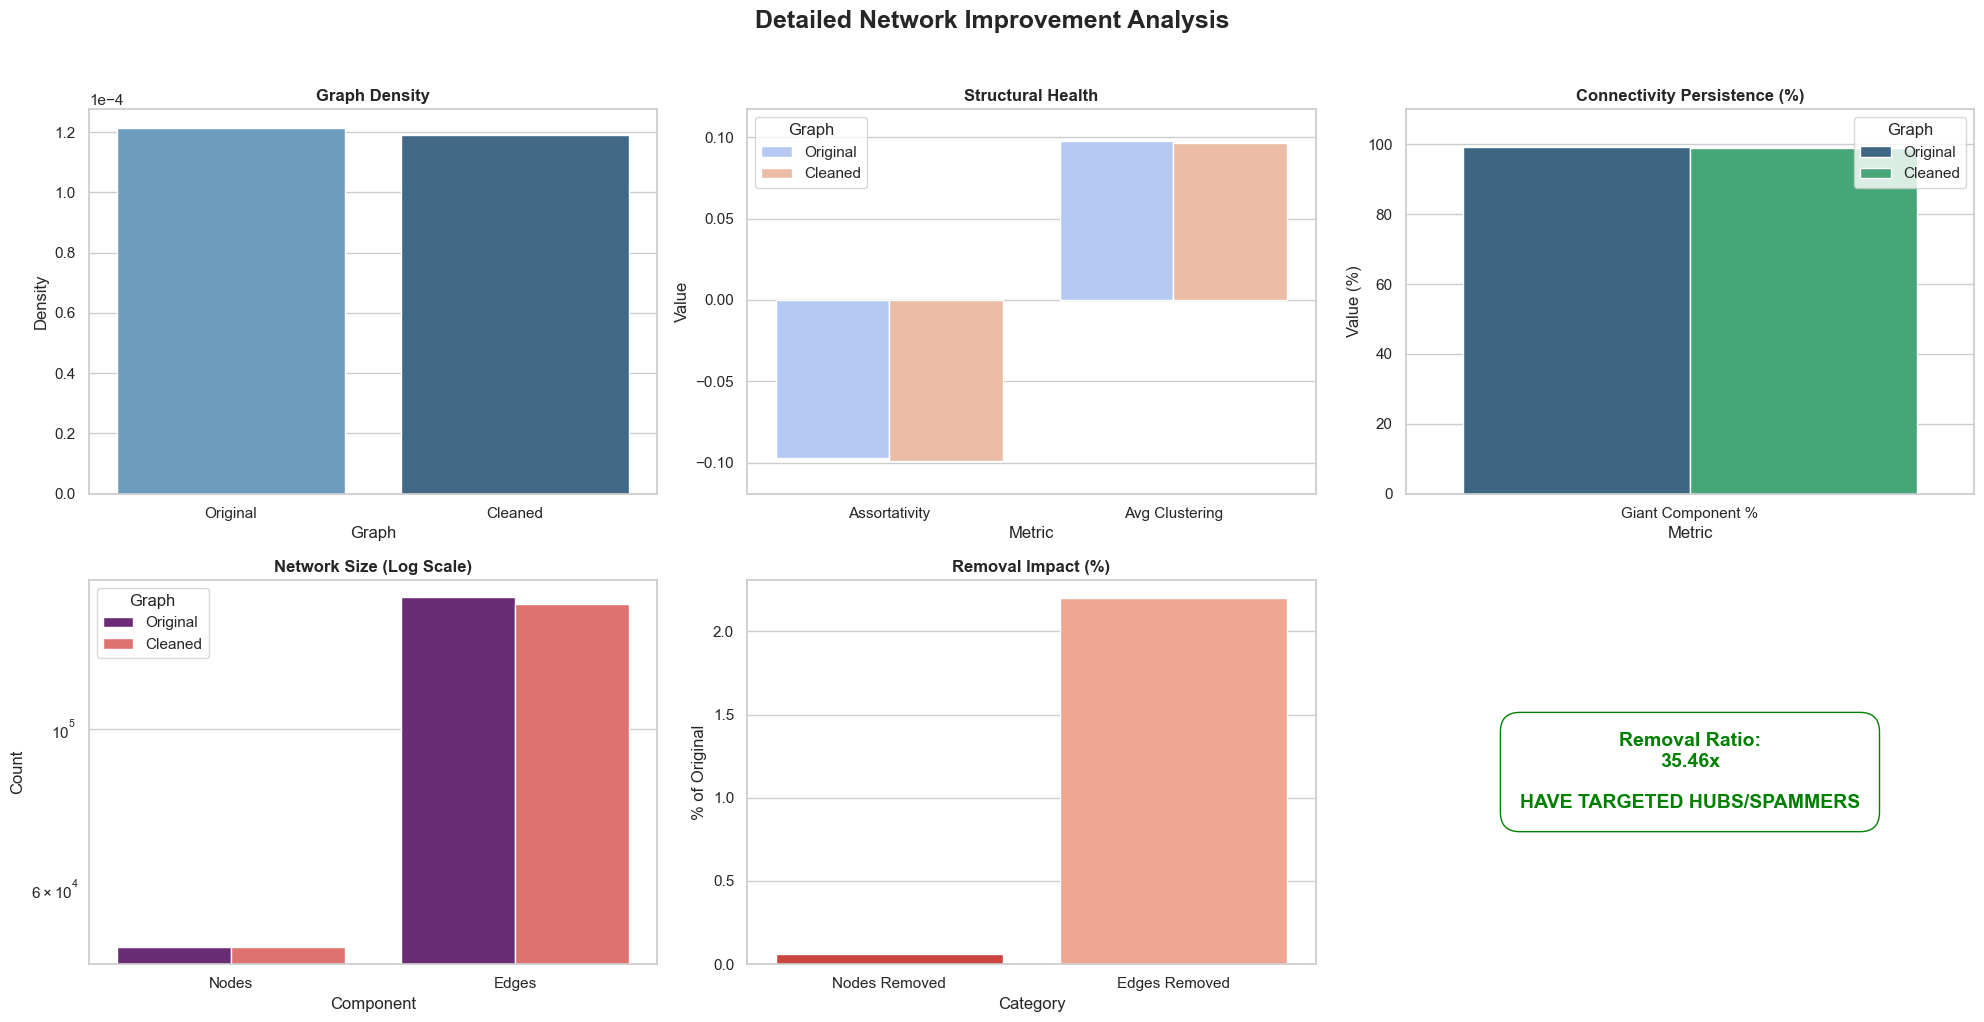
\includegraphics[width=1.0\textwidth]{images/alert_results.png}
    \caption{Résultats pour suppression des alert users.}
    \label{fig:sentiment}
\end{figure}

\end{document}
